\section{Source code}
The source code for this project, licensed under the MIT License, is hosted on \href{https://github.com/Gantzhorn/Thesis}{Github}. In the repository the source code can be found in the \textit{"source\_code"}-directory. To recreate the main results from the thesis run the \code{R}-script: \textit{"main.R"}. The main-file has loads of boilerplate code; if one wants to understand the methods themselves it is easier to read the other \code{R}-files in the same directory. Apart from the code these also includes information about the code as well as minimal examples on how to actually run it. 
\section{Simulation Methods}\label{appendix:simMethods}
This section focuses on constructing the simulation schemes that support the analytical work presented in this thesis. We considered the Euler-maruyama - as well the Milstein scheme. However, as the processes are quite non-linear our final choice was the Scalar weak order 2.0 Itô–Taylor method \cite[algorithm 8.5]{Srkk2019}. In the general setup we simulate $X_0,X_{t_1},\dots, X_{t_N}$ according to the schemes by sampling $N$ random variables $\Delta W_{t_k}\sim\mathcal{N}\left(0, \Delta t_k\right)$. Note that we let $X_{t_0} = \mu_0$, i.e. mean-reverting parameter in the stationary parts of the processes.
\noindent \textbf{Additive noise}\\
Invoking \cite[algorithm 8.5]{Srkk2019} we get the scheme
\begin{align}
    X_{t_{k + 1}} &= X_{t_k} - \left(A(X_{t_k} - m)^2 + \lambda_{t_k}\right) \Delta t_k + \sigma \Delta W_{k} \nonumber \\&-  A \left(X_{t_k} - m\right)\sigma \Delta W_k \Delta t_k\nonumber \\
    & + \left(A\left(X_{t_k} - m\right)\left(A\left(X_{t_k} - m\right)^2 + \lambda_{t_k}\right) - \frac{A \sigma^2}{2}\right)\left(\Delta t_k\right)^2 \label{eq:OUSim}
\end{align}
\\
\textbf{Square-root noise}\\
For the square-root based process the algorithm gives 
\begin{align}
    X_{t_{k + 1}} &= X_{t_k} - \left(A(X_{t_k} - m)^2 + \lambda_{t_k}\right) \Delta t_k + \sigma \sqrt{X_t} \Delta W_{k}\nonumber\\ &+ \frac{1}{4}\sigma^2 \left(\Delta W_k^2 - \Delta t_k\right)     - A\left(X_{t_k} - m\right)\sigma \sqrt{X_{t_k}} W_k \Delta t_k
    \nonumber\\
     &+ \left(A\left(X_{t_k} - m\right)\cdot \left(A\left(X_{t_k} - m\right)^2 + \lambda_{t_k}\right) - \frac{A\sigma^2 X_{t_k}}{2}\right)(\Delta t_k)^2 \nonumber\\
    &- \frac{1}{4\sqrt{X_{t_k}}}\left(\sigma\left(A\left(X_{t_k} - m\right)^2 + \lambda_{t_k}\right) + \frac{1}{4}\sigma^3\right) \left(\Delta W_k \Delta t_k\right)
\end{align}
\\
\textbf{Linear noise}\\
With linear noise we get the simulation scheme
\begin{align}
    X_{t_{k + 1}} &= X_{t_k} - \left(A(X_{t_k} - m)^2 + \lambda_{t_k}\right) \Delta t_k + \sigma X_t \Delta W_{k} \nonumber \\ &
    + \frac{1}{2}\sigma^2 X_{t_k}\left(\Delta W_{k}^2 - \Delta t_k\right) -A(X_{t_k} - m)\sigma X_{t_k} \Delta W_k\Delta t_k \nonumber\\
    & + \left(A\left(X_{t_k} - m\right)\left(A\left(X_{t_k} - m\right)^2 + \lambda_{t_k}\right) - \frac{A\sigma^2X_{t_k}^2}{2}\right)(\Delta t_k)^2 \nonumber \\
    &- \frac{\sigma}{2}\left(A\left(X_{t_k} - m\right)^2 + \lambda_{t_k}\right)\left(\Delta W_{k}\Delta t_k\right).
\end{align}
\\
\textbf{Skew t-distribution}\\
For the t-diffusion based model, we get
\begin{align}
    X_{t_{k + 1}} &= X_{t_k} - \left(A(X_{t_k} - m)^2 + \lambda_{t_k}\right) \Delta t_k + \sigma \sqrt{\left(X_{t_k}^2 + 1\right)} \Delta W_{k} \nonumber\\
    &+ \frac{\sigma^2}{2}X_t \left(\Delta W_{k}^2 - \Delta t_k\right) - A\left(X_{t_k} - m \right)\sigma\sqrt{\left(X_{t_k}^2 + 1\right)}\Delta W_{k}\Delta t_k \nonumber\\
    &+ \left(\left(A\left(X_{t_k} - m \right)^2+\lambda_{t_k}\right)\left(A\left(X_{t_k} - m \right)\right) - \frac{A\sigma^2}{2}\left(X_t^2 + 1\right)\right)\left(\Delta t_k\right)^2 \nonumber\\
    &-\left(\sigma X_{t_k}\left(A\left(X_{t_k} - m \right)^2 + \lambda_{t_k}\right) - \frac{\sigma^3}{2}\right)\frac{\left(\Delta W_{k}\Delta t_k\right)}{2\sqrt{X_{t_k}^2 + 1}} \label{eq:skew_t_sim}
\end{align} 
\\
\textbf{F-distribution}\\
The model with the F-diffusion based model is sampled as
\begin{align}
    X_{t_{k + 1}} &= X_{t_k} - \left(A(X_{t_k} - m)^2 + \lambda_{t_k}\right) \Delta t_k + \sigma\sqrt{X_{t_k}\left(X_{t_k} + 1\right)}\Delta W_k \nonumber \\
    &+ \frac{\sigma^2}{4}\left(2X_{t_k} + 1\right)\left(\Delta W_k^2 - \Delta t_k\right) - A \left(X_{t_k} - m\right)\sigma \sqrt{X_{t_k}\left(X_{t_k} + 1\right)}\Delta W_k \Delta t_k \nonumber \\
    &+ \left(\left(A\left(X_{t_k} - m\right)^2 + \lambda_{t_k}\right)\left(A\left(X_{t_k} - m\right)\right) - \frac{\sigma^2A}{2}\left(X_{t_k}\left(X_{t_k} + 1\right)\right)  \right)\left(\Delta t_k\right)^2 \nonumber \\
    &- \left(\sigma\left(A\left(X_{t_k} - m\right)^2 + \lambda_{t_k}\right)\left(2 X_{t_k} + 1\right) + \frac{\sigma^3}{4}\right)\frac{\Delta W_k \Delta t_k}{4\sqrt{X_{t_k}\left(X_{t_k} + 1\right)}}
\end{align}
\\
\textbf{Jacobi-diffusion}\\
Basing the modelling on the jacobi diffusion yields a scheme
\begin{align}
    X_{t_{k + 1}} &= X_{t_k} - \left(A(X_{t_k} - m)^2 + \lambda_{t_k}\right) \Delta t_k + \sigma \sqrt{X_{t_k}\left(1-X_{t_k}\right)} \Delta W_{k} \nonumber\\
    &+ \frac{\sigma^2}{4}\left(1 - 2X_{t_k}\right)\left(\Delta W_k^2 - \Delta t_k\right) - A\left(X_{t_k} - m\right)\sigma \sqrt{X_{t_k}\left(1 - X_{t_k}\right)}\Delta W_k\Delta t_k \nonumber \\
    &+ \left(\left(A\left(X_{t_k} - m\right)^2 + \lambda_{t_k}\right)\left(A\left(X_{t_k} - m\right)\right) - \frac{\sigma^2A}{2}\left(X_{t_k}\left(1 - X_{t_k}\right)\right)\right)\left(\Delta t_k\right)^2 \nonumber \\
    &- \left(\left(A\left(X_{t_k} - m\right)^2 + \lambda_{t_k}\right)\sigma\left(1 - 2X_{t_k}\right) + \frac{\sigma^3}{2}\right)\frac{\Delta W_k \Delta t_k}{4\sqrt{X_{t_k}\left(1 - X_{t_k}\right)}} \label{eq:jacobiDiffusion}
\end{align}
\section{Derivation of Estimators}\label{sec:AppendixEstim}
In this section, we derive the estimators that have been employed throughout the thesis. For sake of readibility, we leave out some of the more lengthy algebraic manipulations
\subsection{The Ornstein-Uhlenbeck based model}\label{subsec:OUprocess}
This section introduces the estimators for the dynamical system with additive noise. This is the same model introduced in \cite[equation (1)]{Ditlevsen2023} barring the addition of the $\nu$-parameter.
\subsubsection{Stationary part}\label{subsubsec:OUprocessStationary}
In the stationary part of the process we may assume that the process behaves like an Ornstein-Uhlenbeck process. 
\begin{align}
    \mathrm{d}X_t = -\alpha_0\left(X_t-\mu\right) \mathrm{d}t + \sigma \mathrm{d}W_t.
\end{align}
Let $\rho = \exp\left(-\alpha_0\Delta t\right), \gamma^2 = \sigma^2/2\alpha_0$. This process has transition density \cite[equation (S3)]{DitlevsenSupplementary}
\begin{align}
    p\left(\Delta t, x_{i-1}, x_i;\theta\right) = \frac{1}{\sqrt{2\pi\gamma^2\left(1-\rho^2\right)}}\exp\left(-\frac{\left(x_i-x_{i-1}\rho - \mu\left(1-\rho\right)\right)^2}{2\gamma^2\left(1-\rho^2\right)}\right), \label{eq:OULikelihood}
\end{align}
which is a gaussian density with conditional mean and -variance
\begin{align}
    \mathbb{E}\left[X_i\middle|X_{i-1} = x_{i-1}\right] &= x_{i - 1}\rho - \mu\left(1-\rho\right),\\
    \mathrm{Var}\left(X_i\middle|X_{i-1} = x_{i-1}\right) &= \gamma^2\left(1-\rho^2\right).
\end{align}
Unfortunately, we cannot get closed form solution to all of the estimators from this. However, we can still maximize (\ref{eq:OULikelihood}) with respect to $\theta$ to get the MLEs. Alternatively, we can derive the score equations by taking the derivative of the log-likelihood, and numerically solve the non-linear equations we get from doing so. The score equations are present in \cite[p.1, bottom]{DitlevsenSupplementary}. To solve the equations, we use the $\code{nleqslv::nleqslv}$-method \cite{nleqslv}. For starting values in both methods we use the approximation for the MLE of $\mu$ in equation \cite[(S4)]{DitlevsenSupplementary} along with (S4),(S5) for $\rho, \gamma^2$, which are good closed form approximations of the MLEs.
\subsubsection{Dynamic part}\label{subsubsec:OUprocessDynamic}
This part of the estimation procedure has to do with the estimation of the parameters linked to the dynamic part of the process. Our estimation procedure mostly follows \cite{Ditlevsen2023}. We, of course, have the addition of the $\nu$-parameter. Additionally, \cite{Ditlevsen2023} uses regularization in the form of a penalization parameter that punishes values of $A$ significantly smaller than $1$; we do not explore this option here. Recall the dynamics for $t>t_0$
\begin{align}
    \mathrm{d}X_t &= -\left(A\left(X_t - m\right) + \lambda_t\right)\mathrm{d}t + \sigma \mathrm{d}W_t \label{eq:additiveDynamicPart},\\
    \lambda_t &= \lambda_0\left(1 - \frac{t - t_0}{\tau_c}\right)^\nu.
\end{align}
For this part of the process, we utilize the estimation method described in \cite{DitlevsenSupplementary}. The fixed point of the process is $\mu\left(\lambda\right) = \sqrt{-\frac{\lambda_t}{A}}$. Linearizing the process around this value yields the splitting
\begin{align}
    \mathrm{d}X_t^{(1)} &= -\alpha\left(\lambda\right)\left(X_t^{(1)} - \mu\left(\lambda\right)\right)\mathrm{d}t + \sigma \mathrm{d}W_t, \label{eq:additiveSDE}\\
    \mathrm{d}X_t^{(2)} &= -A \left(X_t^{(2)} - \mu\left(\lambda\right)\right)^2\mathrm{d}t. \label{eq:additiveODE}
\end{align}
We recognize the Ornstein-Uhlenbeck process in (\ref{eq:additiveSDE}), for which the solution is (\ref{eq:OU_solution}). Denote this flow $\varphi_{\Delta t}^{(1)}(x)$. Additionally, one can show that (\ref{eq:additiveODE}) is solved by 
\begin{align}
    \varphi^{(2)}_{\Delta t}(x) = \frac{\mu\left(\lambda\right)A\Delta t\left(x - \mu\left(\lambda\right)\right) + x}{A\Delta t\left(x- \mu\left(\lambda\right)\right) + 1}.
\end{align}
By the remark below \cite[equation (9)]{SplittingSchemes} the inverse of the flow is
\begin{align}
    \left(\varphi^{(2)}_{\Delta t}\right)^{-1}(x) = \varphi^{(2)}_{-\Delta t}(x) = \frac{\mu\left(\lambda\right)A\Delta t\left(x - \mu\left(\lambda\right)\right) - x}{A\Delta t\left(x- \mu\left(\lambda\right)\right) - 1},
\end{align}
and by computing the derivative directly
\begin{align}
    \frac{\partial}{\partial x} \left(\left(\varphi^{(2)}_{\Delta t}\right)^{-1}\right)(x) = \frac{1}{\left(A \Delta t\left(x-\mu\left(\lambda \right)\right) - 1\right)^2}.
\end{align}
Then the Strang splitting approximates the transition density of (\ref{eq:additiveDynamicPart}) by
\begin{align}
    \left(X_{t + \Delta t} | X_t = x\right) &= \left(\varphi^{(2)}_{\Delta t / 2}\circ \varphi^{(1)}_{\Delta t} \circ \varphi^{(2)}_{\Delta t / 2}\right) \label{eq:OU_dynamic_likelihood}
\end{align}
This is the transformation of gaussian with appropriate parameters for the mean and variance according to (\ref{linearSDEMean}) and (\ref{linearSDEVariance}) respectively, so we can get the pseudo-loglikelhood using the elements from above and the density transformation theorem. The maximizer of (\ref{eq:OU_dynamic_likelihood}) is then our estimate. 
\subsection{Square-root process}\label{subsec:squareroot}
In this section we introduce the estimators for the model that is based on the square-root process. The estimators for the dynamic part of the process are unlike the ones from the model with additive noise that we showed in \ref{subsec:OUprocess} completely novel
\subsubsection{Stationary part}\label{subsubsec:squarerootStationary}
In the stationary part we assume the process can be modelled by the square-root process
\begin{align}
    \mathrm{d}X_t &= -\alpha_0\left(X_t - \mu_0\right)\mathrm{d}t + \sigma \sqrt{X_t} \mathrm{d}W_t. \label{eq:squarerootAppendix}
\end{align}
We first introduce estimators based on the Strang splitting scheme, and then we consider an estimator based on martingale estimating equations.\\\\
\noindent \textbf{The Strang-based Estimator}\\
To obtain the strang estimator, we first use the lamperti transformation of (\ref{eq:squarerootAppendix}), which by table \ref{table:ergodicDiffusions} is $Y_t := 2\sqrt{X_t}$. To confirm this and get the resulting SDE see
\begin{align}
    \mathrm{d}Y_t = - \frac{2}{Y_t}\left(\alpha_0 \frac{Y_t^2}{4} - \alpha_0 \mu_0 + \frac{\sigma^2}{2}\right)\mathrm{d}t + \sigma \mathrm{d}W_t, \label{eq:lampertiSquarerootAppendix}
\end{align}
by Itô's formula. Then, we use the heuristic from \cite[section 2.3 and 2.5]{SplittingSchemes}. First we calculate the fixed point of the drift. That is, we solve the equation
\begin{align}
    f(y) := - \frac{2}{y}\left(\alpha_0 \frac{y^2}{4} - \alpha_0 \mu_0 + \frac{\sigma^2}{2}\right) = 0
\end{align}
in terms of $y$. By the quadratic formula this is $y^* = \pm 2\sqrt{\frac{\alpha_0\mu_0 - \sigma^2 / 2}{\alpha_0}}$. In our case, however, $Y_t$ is non-negative by definition; thus we only want the positive solution. Therefore, we let the Ornstein-Uhlenbeck part be the linearization around the positive fixed point
\begin{align}
    \mathrm{d}Y_t^{[1]} &= -\alpha_0 \left(Y_t^{[1]} - 2\sqrt{\frac{\alpha_0\mu_0 - \sigma^2 / 2}{\alpha_0}}\right)\mathrm{d}t + \sigma \mathrm{d}W_t , \label{eq:squarerootStationarySplit1} \\
    \mathrm{d}Y_t^{[2]} &= \left(\frac{\alpha_0 Y_t^{[2]}}{2} + \frac{2\alpha_0 \mu_0 - \sigma^2}{Y_t} - 2\sqrt{\alpha_0\left(\alpha_0\mu_0 - \sigma^2 / 2\right)}\right)\mathrm{d}t. \label{eq:squarerootStationarySplit2}
\end{align}
As always, the deterministic ODE in (\ref{eq:squarerootStationarySplit2}) is the residual of (\ref{eq:lampertiSquarerootAppendix}) and (\ref{eq:squarerootStationarySplit1}).
Equation (\ref{eq:squarerootStationarySplit1}) represents an Ornstein-Uhlenbeck process, which with stepsize, $\Delta t$, has a gaussian flow with mean 
\begin{align}
    \mu_{\Delta t}(x) = \exp\left(-\alpha_0 \Delta t\right) \left(x - 2\sqrt{\frac{\alpha_0\mu_0 - \sigma^2 / 2}{\alpha_0}}\right) + 2\sqrt{\frac{\alpha_0\mu_0 - \sigma^2 / 2}{\alpha_0}}
\end{align}
and variance
\begin{align}
     \Omega_{\Delta t} = \frac{\sigma^2\left(1 - \exp\left(-2\alpha_0 \Delta t\right)\right)}{2\alpha_0}
\end{align}
\cite[(5), (6)]{SplittingSchemes}. We did not find an analytical solution to (\ref{eq:squarerootStationarySplit2}) unlike earlier. Instead, we rely  on the classical Fourth-Order Runge-Kutta Method \cite[p. 541]{numericalAnalysis} to find the flow. Nevertheless, we can denote these two flows $\varphi_{\Delta t}^{[1]}, \varphi_{\Delta t}^{[2]}$ respectively and the Strang splitting scheme is then the composition
\begin{align}
    X_{t_{k + 1}} = \left(\varphi_{\Delta t}^{[2]} \circ \varphi_{\Delta t}^{[1]} \circ \varphi_{\Delta t}^{[2]}\right)\left(X_{t_k}\right).
\end{align}
That gives us our psuedo-likelihood; a non-linear transformation of a gaussian random variable. The maximizer of this function is then our estimator. \\\\
\noindent \textbf{Approximate Quadratic Martingale Estimating Equation}\\
We start by deriving the expressions for the one-step ahead conditional mean and variances. The infinitesemal generator (\ref{eq:infinitesemalGeneratorDefinition}) for the square-root process (\ref{eq:squarerootAppendix}) is 
\begin{align}
    \mathcal{L}f = \frac{1}{2}\sigma^2x\frac{\mathrm{d}}{\mathrm{d}x^2}f -\alpha_0\left(x - \mu\right)\frac{\mathrm{d}}{\mathrm{d}x}f. \label{eq:infinitesemalGeneratorSquareRootProcess}
\end{align}
By direct computation one can find 
\begin{align}
    \phi_1(x) &= x-\mu, &&\; \lambda_1 = \alpha_0, \label{squarerooteigen1}\\
    \phi_2(x) &= x^2 - \left(2\mu + \frac{\sigma^2}{\alpha_0}\right)x + \mu^2 + \frac{\sigma^2\mu}{2\alpha_0}, &&\; \lambda_2 = 2\alpha_0. \label{squarerooteigen2}
\end{align}
For completeness, we verify these results by inserting into (\ref{eq:infinitesemalGeneratorSquareRootProcess})
\begin{align}
    \mathcal{L}\phi_1(x) = -\alpha_0\left(x - \mu\right)\cdot 1 + \frac{1}{2}\sigma^2 x \cdot 0 = -\alpha_0\left(x - \mu\right) = -\lambda_1\phi_1(x). \label{eq:directVerificationCondMean}
\end{align}
Additionally,
\begin{align}
    \mathcal{L}\phi_2(x) &= -\alpha_0\left(x - \mu\right)\cdot \left(2x -2\mu - \frac{\sigma^2}{\alpha_0}\right) + \sigma^2x\\
    =& -2\alpha_0\left(x^2-x\mu - x\mu + \mu^2 -\frac{\sigma^2}{2\alpha_0}x + \frac{\sigma^2}{2\alpha_0}\mu - \frac{\sigma^2}{2\alpha_0}x \right)\\
    &= -2\alpha_0 \left(x^2 -\left(2\mu+\frac{\sigma^2}{\alpha_0}\right)x + \mu^2 + \frac{\sigma^2\mu}{2\alpha_0}\right) = -\lambda_2\phi_2(x).\\
\end{align}
Now using (\ref{eq:momentConditions}) the conditional mean can be calculated as
\begin{align}
    E\left[X_{\Delta t} - \mu \middle| X = x\right] &= \exp\left(-\alpha_0\Delta t\right)\left(x-\mu\right),\\
    E\left[X_{\Delta t} \middle| X = x\right] &= \exp\left(-\alpha_0\Delta t\right)\left(x-\mu\right) + \mu. \label{eq:squarerootCondMean}
\end{align}
Similarly, the conditional one-step ahead second moment is found
\begin{align}
    &\mathbb{E}\left[X_{\Delta t}^2 - \left(2\mu + \frac{\sigma^2}{\alpha_0}\right)X_{\Delta t} + \mu^2 + \frac{\sigma^2\mu}{2\alpha_0} \middle| X = x \right] \nonumber \\
    &= \exp\left(-2\alpha_0 \Delta t\right)\left(x^2 - \left(2\mu + \frac{\sigma^2}{\alpha_0}\right)x + \mu^2 + \frac{\sigma^2 \mu}{2\alpha_0}\right),\\
    \mathbb{E}\left[X_{\Delta t}^2 \middle| X = x\right] &= \exp\left(-2\alpha_0 \Delta t\right)\left(x^2 - \left(2\mu + \frac{\sigma^2}{\alpha_0}\right)x + \mu^2 + \frac{\sigma^2 \mu}{2\alpha_0}\right)  \nonumber  \\
     &+ \left(2\mu + \frac{\sigma^2}{\alpha_0}\right) \left(\exp\left(-\alpha_0\Delta t \right)\left(x-\mu\right) + \mu\right) - \left(\mu^2 + \frac{\sigma^2\mu}{2\alpha_0}\right). \label{eq:squarerootCondsecondMoment}
\end{align}
By definition of conditional variance and combining (\ref{eq:squarerootCondsecondMoment}) and (\ref{eq:squarerootCondMean}), one easily gets
\begin{align}
    \mathrm{Var}\left(X_{\Delta t} \middle| X = x \right) = \frac{\sigma^2}{\alpha_0}\left(\exp\left(-2\alpha_0\Delta t \right)\left(\frac{\mu}{2} - x   \right) - \exp\left(-\alpha_0\Delta t\right)\left(\mu - x\right) + \frac{\mu}{2}\right). \label{eq:squarerootCondVariance}
\end{align}
Denote the conditional mean and -variance, $F_i, \Phi_i$, respectively. We get by using (\ref{eq:approximatelyOptimalMartingale}) an approximate quadratic martingale estimation equation
\begin{align}
        G_N^{sq} = \begin{bmatrix}
            \sum_{i = 1}^N \frac{\alpha_0}{\sigma^2 X_{t_{i-1}}}\left(X_{t_i} - F_{t_i}\right)\\
            \sum_{i = 1}^N \frac{-1}{\sigma^2}\left(X_{t_i} - F_{t_i}\right)\\
            \sum_{i = 1}^N \frac{1}{\sigma^3 X_{t_{i-1}}}\left(\left(X_{t_i} - F_{t_i}\right)^2 - \Phi_{t_i}\right) \label{eq:squarerootMartingaleEquation}
        \end{bmatrix}.
\end{align}
Setting $G_N^{sq} = 0$ we get the following explicit estimators
\begin{align}
    \exp\left(-\hat{\alpha_0}_N\Delta\right) &= \frac{N\sum_{i=1}^{N}X_{t_i} / X_{t_{i - 1}} - \left(\sum_{i = 1}^{N}X_{t_i}\right)\left(\sum_{i}^{N}1/X_{t_{i - 1}}\right)}{N^2 - \left(\sum_{i = 1}^{n}X_{t_i}\right)\left(1/X_{t_{i - 1}}\right)},\\
    \hat{\mu}_N &= \frac{\sum_{i = 1}^{N}X_{t_i} / X_{t_{i - 1}} - N \exp\left(-\hat{\alpha_0}_N\Delta\right)}{\left(1-\exp\left(-\hat{\alpha_0}_N\Delta\right)\right)\sum_{i = 1}^{N}1/X_{t_{i - 1}}}.
\end{align}
For the two parameters related to the drift of the process. Now, define
\begin{align}
    \Phi^*(\Delta, x; \theta) := \left(\frac{x}{\alpha_0}\left(\exp\left(-\alpha_0\Delta - \exp\left(-2\alpha_0 \Delta\right)\right)\right) + \frac{\mu}{2\alpha_0}\left(1-\exp\left(-\alpha_0\Delta\right)\right)^2\right).
\end{align}
Then the third equation in (\ref{eq:squarerootMartingaleEquation}) yields the explicit equation for the noise-parameter
\begin{align}
    \hat{\sigma}^2_N = \frac{\sum_{i = 1}^{N}\frac{1}{X_{t_{i - 1}}}\left(X_{t_i} - F_i\right)^2}{\sum_{i = 1}^{N}\frac{1}{X_{t_{i - 1}}}\Phi^*(\Delta, x; \theta)}
\end{align}
\subsubsection{Dynamic part}\label{subsubsec:squarerootDynamic}
In its dynamic part the process, we assumed that the model is governed by the stochastic differential equation
\begin{align}
    \mathrm{d}X_t &= -\left(A\left(X_t - m\right) + \lambda_t\right)\mathrm{d}t + \sigma \sqrt{X_t} \mathrm{d}W_t, \label{eq:dynamicsquarerootSDE}\\
    \lambda_t &= \lambda_0\left(1 - \frac{t - t_0}{\tau_c}\right)^\nu.
\end{align}
And as usual we assume that we already estimations from the stationary part i.e. that $\lambda_0, \sigma, m$ are available. That is from \ref{subsubsec:squarerootStationary} we have the estimates $\alpha_0, \mu_0, \sigma$ and we can compute
\begin{align}
    m &= \mu_0 - \frac{\alpha_0}{2A},\\
    \lambda_0 &= - \frac{\alpha_0^2}{4A}.
\end{align}
In other words, our objective is to estimate $A, \tau_c, \nu$, where $\tau_c$ obviously is our parameter of interest. The drift term is the same as in \cite{Ditlevsen2023}, thus in complete analogy to \cite[(S9, S10)]{DitlevsenSupplementary} we split the system into
\begin{align}
    \mathrm{d}X_t^{[1]} &= -\alpha(\lambda)\left(X_t^{[1]} - \mu(\lambda)\right)  \mathrm{d}t + \sigma \sqrt{X_t^{[1]}} \mathrm{d}W_t, \label{eq:squareRootSplit1} \\
    \mathrm{d}X_t^{[2]} &= - A \left(X_t^{[2]} - \mu(\lambda)\right)^2 \mathrm{d}t, \label{eq:squareRootSplit2}
\end{align}
with $\alpha(\lambda) = 2\sqrt{\abs{A\lambda_t}}$ and $\mu(\lambda) = m + \sqrt{-\frac{\lambda_t}{A}}$.
This particular choice of splitting is done by letting the square-root process part be the linearization around the fixed point of the process. It is evident that equation (\ref{eq:squareRootSplit2}) is identical to equation \cite[(S10)]{DitlevsenSupplementary}; thus the flows are the same.\\ However, the square-root dependency in the noise-term (\ref{eq:squareRootSplit1}) yields a flow that is different to the flow of \cite[(S9)]{DitlevsenSupplementary}. To address this, we adopt the approach developed by Kessler \cite{Kessler1997} to (\ref{eq:squareRootSplit1}). Kessler's method approximates the transition density by a gaussian density using the true conditional mean and- variance. The process, (\ref{eq:squareRootSplit1}), is the square-root process, for which we found exactly these quantities (\ref{eq:squarerootCondMean}) and (\ref{eq:squarerootCondVariance}). Denote the flow with steplength, $\Delta t$, of \ref{eq:squareRootSplit1} and \ref{eq:squareRootSplit2} $\varphi_{\Delta t}^{(1)}, \varphi_{\Delta t}^{(2)}$ respectively, then the Strang based flow is 
\begin{align}
    \left(X_{t_n + \Delta t} | X_{t_n} = x\right) = \left(\varphi_{\Delta t/2}^{(2)} \circ \varphi_{\Delta t}^{(1)} \circ \varphi_{\Delta t/2}^{(2)}\right)(x),
\end{align} 
which gives rise to a pseudo-likelihood similar to \cite[(14)]{SplittingSchemes}. The maximizer of the pseudo-likelihood is the Strang-based estimator.
On the other hand, we can also use the regular Strang-likelihood that uses a splitting based on (\ref{SDE_split}) and (\ref{ODE_Split}). The lamperti-transform only depends on the noise term and therefore (\ref{eq:dynamicsquarerootSDE}) has the same lamperti-transform as the square-root process. Let $Y_t:= 2\sqrt{X_t}$ and use Itô's formula on (\ref{eq:dynamicsquarerootSDE}), then
\begin{align}
    \mathrm{d}Y_t = - \frac{2}{Y_t}\left(A\left(\frac{Y_t^2}{4} - m\right)^2 + \lambda_t + \frac{\sigma^2}{4}\right)\mathrm{d}t + \sigma \mathrm{d}W_t. \label{eq:lampertiTransformedDynamicSquareroot}
\end{align}
Linearizing this around the fixed point of the drift, we get the following splitting scheme
\begin{align}
    \mathrm{d}Y_t^{[1]} &= A_{\mathrm{linear\_part}}\left(Y_t^{[1]} - b_{\mathrm{intercept}}\right)\mathrm{d}t + \sigma \mathrm{d}W_t, \label{eq:lampertiSquarerootSplitting1}\\
    \mathrm{d}Y_t^{[2]} &= - \left(\frac{2}{Y_t^{[2]}}\left(A\left(\frac{\left(Y_t^{[2]}\right)^2}{4} - m\right)^2 + \lambda_t + \frac{\sigma^2}{4}\right) + A_{\mathrm{linear\_part}}\left(Y_t^{[2]} - b_{\mathrm{intercept}}\right)\right)\mathrm{d}t,
\end{align}
where we use the following quantities
\begin{align}
    A_{\mathrm{linear\_part}} &= -\sqrt{-A\left(4\lambda_t + \sigma^2\right)},\\
    b_{\mathrm{intercept}} &= 2 \sqrt{\frac{Am + \sqrt{-A\left(\lambda_t + \sigma^2/4\right)}}{A}},
\end{align}
note that $b_{\mathrm{intercept}}$ is the fixed point of the drift in (\ref{eq:lampertiTransformedDynamicSquareroot}). Not surprisingly, this quantity as well as the slope of the linear SDE indirectly depends on time through $\lambda_t$. \\
We solve these flows using the solution to the Ornstein-Uhlenbeck process and a fourth-order Runge-kutta respectively. The solutions in the usual composition of (\ref{eq:classicStrangSplitting}) then gives us the Strang-flow, which we maximize in order to get the Strang-based estimator for the lamperti-transformed process.
\subsection{Mean-reverting Geometric Brownian Motion}\label{subsec:meanrevertingGBM}
This section derives the estimators for the stationary- and non-stationary part of the model based on the noise term from the mean-reverting geometric brownian motion.
\subsubsection{Stationary part}\label{subsubsec:meanrevertingGBMStationary}
In the stationary part we assume the process can be modelled by the mean-reverting Geometric Brownian Motion.
\begin{align}
    \mathrm{d}X_t &= -\alpha_0\left(X_t - \mu_0\right)\mathrm{d}t + \sigma X_t \mathrm{d}W_t \label{eq:GBM_simple}
\end{align}
For this process we present three estimation methods in total. The first two methods are based on the Strang splitting scheme, whereas the second is a an approximately optimal martingale estimation equation \\
\noindent \textbf{Strang splitting estimators}\\
Here we present two estimators based on different splitting philosophies. First we consider a naïve splitting. That is, we split the mean-reverting GBM into
\begin{align}
    \mathrm{d}X_t^{[1]} &= \sigma X_t^{[1]}\mathrm{d}W_t, \; &&X_{t_0} = x_0, \label{meanrevertingGBMSplit1}\\
    \mathrm{d}X_t^{[2]} &= -\beta\left(X_t^{[2]} - \mu\right)\mathrm{d}t, \; &&X_{t_0} = x_0. \label{meanrevertingGBMSplit2}
\end{align}
With stepsize, $\Delta t$, (\ref{meanrevertingGBMSplit1}) has solution according to \cite[example 4.7]{Srkk2019}
\begin{align}
    X_{t_0 + \Delta t}^{[1]} = \exp\left(\log(x_0) -\frac{\sigma^2}{2}\Delta t + \sigma \Delta W_t\right).
\end{align}
Because $\Delta W_t\sim\mathcal{N}(0,\Delta t)$, this flow is log-normal with parameters $\mu_{\mathrm{log}} = \log(x_0) -\frac{\sigma^2}{2}\Delta t$ and $\sigma_{\log} = \sigma^2\Delta t$ respectively. For typographical reasons, denote this solution $\varphi_{\Delta t}^{[1]}(x_0)$. Now, we find the solution to the ODE (\ref{meanrevertingGBMSplit2}), along with its inverse 
\begin{align}
    f_{\Delta t}(x_0) &= (x_0 - \mu)\exp(-\beta\Delta t) + \mu \label{eq:meanRevertingODESolution}\\
    f_{\Delta t}^{-1}(x_1) &=  (x_1 - \mu)\exp(\beta\Delta t) + \mu\\
    \frac{\partial}{\partial x} f_{\Delta t}^{-1}(x_1) &= \exp\left(\beta\Delta t\right).
\end{align}
The inverse is calculated with \cite[remark belown equation (9)]{SplittingSchemes}. Let $\varphi_{\Delta t}^{[2]}(x_0)$ be the flow described by (\ref{eq:meanRevertingODESolution}).
The Strang splitting scheme is the composition
\begin{align}
    \left(X_{t_0 + \Delta t} | X_{t_0}\right) = \left(\varphi_{\Delta t / 2}^{[2]}\circ \varphi_{\Delta t}^{[1]} \circ \varphi_{\Delta t / 2}^{[2]}\right)(x_0)
\end{align}
This is the transformation given by (\ref{eq:meanRevertingODESolution}) of a log-normal random variable. This yields a Strang based negative pseudo log-likelihood
\begin{align}
    l_S(\beta, \mu, \sigma) = \sum_{i = 1}^{N} g(f_{\Delta t}^{-1}(x_i); \beta,\mu, \sigma) - \frac{\beta\Delta t(N - 1)}{2},
\end{align}
where $g$ is minus the logarithm of the log-normal density with parameters, $\mu_{\mathrm{log}}$ and $\sigma_{\mathrm{log}}$, and $N$ the number of samples.\\
Conversely, we can use the lamperti transformation of the mean-reverting GBM and the familiar Strang likelihood (\ref{eq:Strang_likelihood}). The lamperti transform of (\ref{eq:GBM_simple}) is $Y_t = \log(X_t)$ and by Itôs formula the resulting SDE is
\begin{align}
    \mathrm{d}Y_t = -\left(\beta\left(1 - \mu\exp(-Y_t)\right) + \frac{1}{2}\sigma^2\right)\mathrm{d}t + \sigma \mathrm{d}W_t. \label{eq:GBM_lamperti}
\end{align}
The fixed point of the drift in (\ref{eq:GBM_lamperti}) is $-\log\left(\frac{\sigma^2 + 2\beta}{2\beta\mu}\right)$. We use the well-known heuristic from \cite{SplittingSchemes} and linearize around the fixed-point to get the splitting
\begin{align}
    \mathrm{d}Y_t^{[1]} &= - \frac{\sigma^2 + 2\beta}{2}\left(Y_t^{[1]} + \log\left(\frac{\sigma^2 + 2\beta}{2\beta \mu}\right)\right)\mathrm{d}t + \sigma \mathrm{d}W_t, \label{eq:GBM_LinearSDE_split}\\
    \mathrm{d}Y_t^{[2]} &= \left(-\beta + \beta\mu\exp(-Y_t^{[2]}) - \frac{\sigma^2}{2} + \frac{\sigma^2+2\beta}{2}Y_t^{[2]} + \frac{\sigma^2+2\beta}{2}\log\left(\frac{\sigma^2+2\beta}{2\beta\mu}\right)\right)\mathrm{d}t, \label{eq:GBM_StrangNonLinearODE_split}
\end{align}
where (\ref{eq:GBM_StrangNonLinearODE_split}) is the residual of (\ref{eq:GBM_lamperti}) and (\ref{eq:GBM_LinearSDE_split}).
These flows we solve using the linear SDE and a fourth order Runge-kutta respectively. And then by the composition that defines the Strang flow, we get a approximation for the transition density and a result a pseudo-likelihood, we can maximize.

\noindent \textbf{Approximate Quadratic Martingale Estimating Equation}\\
\noindent Starting once more with deriving the one-step ahead conditional mean and - variance. The generator is
\begin{align}
    \mathcal{L}\varphi = -\beta\left(x - \mu\right)\frac{\mathrm{d}}{\mathrm{d}x}\varphi + \frac{1}{2}\sigma^2 x^2 \frac{\mathrm{d}^2}{\mathrm{d}x^2}\varphi,
\end{align}
whence we get the eigen functions and -values.
\begin{align}
    \varphi_1(x) &= x - \mu, \qquad &&\lambda_1 = \beta, \label{GBMeigen1} \\
    \varphi_2(x) &= x^2 - \frac{2\beta\mu}{\beta - \sigma^2}x + \frac{2\mu^2\beta^2}{\left(\beta - \sigma^2\right)\left(2\beta - \sigma^2\right)}, \qquad &&\lambda_2 = 2\beta - \sigma^2 \label{GBMeigen2}.
\end{align}
Evidently, (\ref{GBMeigen1}) is identical to (\ref{squarerooteigen1}), thus the one-step ahead conditional means are too. Commencing, we now verify that (\ref{GBMeigen2}) is the second eigen function and -value
\begin{align}
    \mathcal{L}\varphi_2 & = -\beta\left(x-\mu\right)\left(2x - \frac{2\beta\mu}{\beta-\sigma^2}\right) + \sigma^2x^2,\\
    &=-\left(2\beta - \sigma^2\right)x^2 + \frac{2\beta\mu\left(2\beta-\sigma^2\right)}{\beta - \sigma^2}x - \frac{2\beta^2\mu^2}{\beta - \sigma^2}, \\
    &= -\left(2\beta -\sigma^2\right)\left(x^2 - \frac{2\beta\mu}{\beta-\sigma^2} + \frac{2\beta^2\mu^2}{\left(\beta-\sigma^2\right)\left(2\beta-\sigma^2\right)}\right),\\
    &= - \lambda_2 \varphi_2.
\end{align}
Therefore, we can calculate the one-step ahead conditional second moment by
\begin{align}
    \mathbb{E}\left[\varphi_2(X_\Delta)\middle|X = x\right] &= \exp\left(-\left(2\beta - \sigma^2\right)\right)\varphi_2(x),
\end{align}
and thus
\begin{align}
    \mathbb{E}\left[X_\Delta^2 \middle| X = x\right] &= \exp\left(-\left(2\beta - \sigma^2\right)\right)\varphi_2(x) + \frac{2\beta\mu}{\beta-\sigma^2} \mathbb{E}\left[X_\Delta\middle|X=x\right] \nonumber \\
    &\quad - \frac{2\beta^2\mu^2}{\left(\beta-\sigma^2\right)\left(2\beta-\sigma^2\right)} \label{GBM_secondmoment}
\end{align}
Now since 
\begin{align}
    \left(\mathbb{E}\left[X_\Delta\middle|X=x\right]\right)^2 &= \left(\exp\left(-\beta\Delta\right)\left(x-\mu\right) + \mu\right)^2 \nonumber\\
    &= \exp\left(-2\beta\Delta\right)\left(x-\mu\right)^2 + \mu^2 + 2\mu\exp\left(-\beta\Delta\right)\left(x-\mu\right). \label{GBM_firstmoment_square}
\end{align}
We get the desired result by combining (\ref{GBM_secondmoment}) and (\ref{GBM_firstmoment_square}) and using the definition of conditional variance
\begin{align}
    \mathrm{Var}\left(X_\Delta \middle| X = x\right) &= \exp\left(-\left(2\beta - \sigma^2\right)\Delta\right)\left(x^2 - \frac{2\beta\mu}{\beta-\sigma^2}x + \frac{2\beta^2 \mu^2}{\left(\beta-\sigma^2\right)\left(2\beta - \sigma^2\right)}\right) \nonumber \\
    &+ \frac{2\beta\mu}{\beta-\sigma^2}\left(\exp\left(-\beta\Delta\right)\left(x-\mu\right) + \mu\right) - \frac{2\beta^2\mu^2}{\left(\beta-\sigma^2\right)\left(2\beta - \sigma^2\right)} \nonumber\\
    &- \exp\left(-2\beta\Delta\right)\left(\left(x-\mu\right)^2 - \mu^2 - 2\mu\exp\left(-\beta\Delta\right)\left(x-\mu\right)\right)
\end{align} 
Denote the one-step ahead conditional mean and -variance $F_i, \Phi_i$ respectively. Now, utilizing the method described in section \ref{subsubsec:approximatelyOptimalMartingaleEstimationEquation} we have approximate quadratic martingale estimation equations given by
\begin{align}
    G_N^{GBM} = \begin{bmatrix}
        \sum_{i = 1}^N \frac{\beta}{\sigma^2 X_{t_{i-1}}^2}\left(X_{t_i} - F_{t_i}\right)\\
        \sum_{i = 1}^N \frac{-1}{\sigma^2 X_{t_{i-1}}}\left(X_{t_i} - F_{t_i}\right)\\
        \sum_{i = 1}^N \frac{1}{\sigma^3 X_{t_{i-1}}^2}\left(\left(X_{t_i} - F_{t_i}\right)^2 - \Phi_{t_i}\right)
    \end{bmatrix}. \label{eq:GBMapproxOptimalMartingaleEstimationEquation}
\end{align}
Solving the equation $G_N^{GBM} = 0$ then yields the approximate quadratic marginale estimator. We were not able able to find closed-form expression for the estimates from the equation this time. Instead, we solved (\ref{eq:GBMapproxOptimalMartingaleEstimationEquation}) numerically using the \code{nleqslv::nleqslv}-method\cite{nleqslv}.
\subsubsection{Dynamic part}\label{subsubsec:meanrevertingGBMDynamic}
In its dynamic part the model with the same noise as the mean-reverting geometric brownian motion is modelled using the stochastic differential equation
\begin{align}
    \mathrm{d}X_t &= -\left(A\left(X_t - m\right) + \lambda_t\right) + \sigma X_t \mathrm{d}W_t, \label{eq:GBM_dynamic_SDE}\\
    \lambda_t &= \lambda_0\left(1 - \frac{t - t_0}{\tau_c}\right)^\nu,
\end{align}
and as in section \ref{subsubsec:squarerootDynamic} we assume that we have estimated $\lambda_0, \sigma, m$ or are able to compute them from other parameters in the same manner. Initially we explore the same choice of splitting as we also started with section \ref{subsubsec:squarerootDynamic}
\begin{align}
    \mathrm{d}X_t^{[1]} &= -\alpha(\lambda)\left(X_t^{[1]} - \mu(\lambda)\right)  \mathrm{d}t + \sigma X_t^{[1]} \mathrm{d}W_t, \label{eq:GBMSplit1} \\
    \mathrm{d}X_t^{[2]} &= - A \left(X_t^{[2]} - \mu(\lambda)\right)^2 \mathrm{d}t, \label{eq:GBMSplit2}
\end{align}
with $\alpha(\lambda) = 2\sqrt{\abs{A\lambda_t}}$ and $\mu(\lambda) = m + \sqrt{-\frac{\lambda_t}{A}}$.
Again, this splitting is obtained by letting the mean-reverting GBM be the linearization around the fixed point of the drift in (\ref{eq:GBMSplit1}). To get the Strang estimator we simply use kessler's method on the mean-reverting GBM in (\ref{eq:GBMSplit1}); we again have the conditional mean- and variance at our disposal. The flow for (\ref{eq:GBMSplit2}) is naturally identical to the one in (\ref{eq:squareRootSplit2}). Finally, the Strang approximation of the transition density is constructed in the usual manner. The maximizer of the resulting pseudo-likelihood is once more the Strang-based estimator.\\
However, as we did with the square-root process, we also explore the option of finding a Strang estimator based on splitting the lamperti-transformed process. For sake of notation let
\begin{align}
    \zeta &= \frac{2mA - \frac{1}{2}\sigma^2 + \sqrt{\sigma^4/4 - A\left(2m\sigma^2 + 4\lambda_t\right)}}{2A},\\
    A_{\mathrm{linear\_part}} &= - \frac{1}{\zeta}\left(A \zeta^2 - \lambda_t - Am^2\right).
\end{align}
As in the stationary part (\ref{eq:GBM_dynamic_SDE}) has lamperti transform $Y_t:=\log(X_t)$. Therefore, we get from Itô's formula
\begin{align}
    \mathrm{d}Y_t = - \left(\frac{A\left(\exp\left(Y_t\right)-m\right)^2 + \lambda_t}{\exp(Y_t)} + \frac{\sigma^2}{2}\right)\mathrm{d}t + \sigma \mathrm{d}W_t \label{eq:GBMdynamicLamperti}
\end{align}
The fixed point of the drift in (\ref{eq:GBMdynamicLamperti}) is $\log\left(\zeta\right)$. We linearize the process around this point to get the following splitting scheme
\begin{align}
    \mathrm{d}Y_t^{[1]} &= A_{\mathrm{linear\_part}}\left(Y_t^{[1]} - \log\left(\zeta\right)\right)\mathrm{d}t + \sigma \mathrm{d}W_t,\\
    \mathrm{d}Y_t^{[2]} &= \left(-\frac{A\left(\exp\left(Y_t^{[2]}\right)-m\right)^2 + \lambda_t}{\exp\left(Y_t^{[2]}\right)} - \frac{\sigma^2}{2}%\right. \nonumber \\
    - A_{\mathrm{linear\_part}}\left(Y_t^{[2]} - \log\left(\zeta\right)\right)\right)\mathrm{d}t. \label{eq:GBMLampertiBasedStrang}
\end{align}
We solve the linear SDE using (\ref{eq:OU_solution}). The non-linear ODE's solution, the inverse of the solution and the derivative of the inverse of the solution will be found numerically with the fourth-order Runge-kutta. Putting together the pieces as (\ref{eq:classicStrangSplitting}); we get the strang-estimator of the lamperti-transformed process in the typical manner.
\subsection{Skew t-distribution}
In this section we introduce the estimators for the model, where the noise is assumed to correspond to a pearson diffusion with stationary distribution equal to the Skew t-distribution.
\subsubsection{Stationary part}
The process with the same noise as the skew t-distribution pearson diffusion is assumed to be governed by this diffusion in the non-dynamic part
\begin{align}
    \mathrm{d}X_t = -\alpha_0\left(X_t - \mu\right)\mathrm{d}t + \sigma \sqrt{\left(X_t^2 + 1\right)}\mathrm{d}W_t.
\end{align}
For estimation of the parameters in the diffusion, we use the Strang splitting. Define $Y_t := \sinh^{-1}(X_t)$, then by Itô's formula
\begin{align}
    \mathrm{d}Y_t = - \frac{1}{\cosh(Y_t)}\left(\sinh(Y_t)\left(\alpha_0 + \frac{1}{2}\sigma^2\right) - \mu\alpha_0\right)\mathrm{d}t + \sigma \mathrm{d}W_t.
\end{align}
The fixed point of this process is $\sinh^{-1}(\frac{2\alpha_0\mu}{2\alpha_0 + \sigma^2})$. With the same splitting method as we have used the majority of the times, we get the splitting scheme
\begin{align}
    \mathrm{d}Y_t^{[1]} &= -\left(\alpha_0 + \frac{1}{2}\sigma^2\right)\left(Y_t^{[1]} - \sinh^{-1}\left(\frac{2\alpha_0\mu}{2\alpha_0 + \sigma^2}\right)\right)\mathrm{d}t + \sigma \mathrm{d}W_t \\
    \mathrm{d}Y_t^{[2]} &= \left(\left(\alpha_0 + \frac{1}{2}\sigma^2\right) \left(Y_t^{[2]} - \tanh\left(Y_t^{[2]}\right) - \sinh^{-1}\left(\frac{2\alpha_0\mu}{2\alpha_0 + \sigma^2}\right)\right) + \right. \nonumber \\
    &\left. \frac{\mu\alpha_0}{\cosh\left(Y_t^{[2]}\right)}\right)\mathrm{d}t, \label{eq:StrangTDiffusion}
\end{align}
and from the solutions to this linear SDE and non-linear ODE, we construct the Strang approximation of the transition density; and thereby its pseudo-likelihood, which we maximize to get the Strang based estimators.
\subsubsection{Dynamic part}
With estimates for $\alpha_0, \mu, \sigma$ we continue by turning to the dynamic part of the process: We want to estimate $A, \tau_c, \nu$ in
\begin{align}
    \mathrm{d}X_t &= -\left(A(X_t - m)^2 + \lambda_t\right)\mathrm{d}t + \sigma \sqrt{\left(X_t^2 + 1\right)}\mathrm{d}W_t,\\
    \lambda_t &= \lambda_0 \left(1 - \frac{t - t_0}{\tau_c}\right)^\nu.
\end{align}
Once again, we use the lamperti-transform: Let $Y_t = \sinh^{-1}(X_t)$; we get from Itô's formula that
\begin{align}
    \mathrm{d}Y_t = -\frac{1}{\cosh(Y_t)}\left(A\left(\sinh(Y_t) - m\right)^2 + \lambda_t + \frac{\sigma^2}{2}\sinh(Y_t)\right)\mathrm{d}t + \sigma \mathrm{d}W_t. \label{eq:LampertiTDistributionDynamic}
\end{align}
For typographical reasons, define
\begin{align}
    A_{\textrm{linear\_part}} &= -\sqrt{\frac{\sigma^4}{4} - 2A\left(2\lambda_t + m\sigma^2\right)}\\
    b_{\textrm{intercept}} &= \sinh^{-1}\left(\frac{\sqrt{\sigma^4 - 8A\left(2\lambda_t + m \sigma^2\right)} + 4 Am - \sigma^2}{4A}\right).
\end{align}
Note that $b_{\textrm{intercept}}$ is the fixed point of (\ref{eq:LampertiTDistributionDynamic}). Linearizing the SDE around this point and computing the non-linear ODE residually yields the following splitting
\begin{align}
    \mathrm{d}Y_t^{[1]} &= A_{\textrm{linear\_part}}\left(Y_t^{[1]} - b_{\textrm{intercept}}\right)\mathrm{d}t + \sigma \mathrm{d}W_t \label{eq:linearSplitTdist} \\
    \mathrm{d}Y_t^{[2]} &= \left(-\frac{1}{\cosh(Y_t^{[2]})}\left(A\left(\sinh(Y_t^{[2]}) - m\right)^2 + \lambda_t + \frac{\sigma^2}{2}\sinh(Y_t^{[2]})\right)\right.\\
     &\left.- A_{\textrm{linear\_part}}\left(Y_t^{[2]} - b_{\textrm{intercept}}\right)\right)\mathrm{d}t \label{eq:StrangTDiffusionDynamic}
\end{align}
We solve (\ref{eq:linearSplitTdist}) using the solution to the OU-process, whereas the solution to the non-linear ODE along with its inverse and derivative of inverse is found numerically with the fourth order Runge-kutta.
\subsection{The scaled F-distribution}
Here we introduce how we construct the estimators for the model that is based on the pearson diffusion that has the scaled F-distribution as its stationary distribution. 
\subsubsection{Stationary part}
In the stationary part of the process the pearson diffusion with the scaled F-distribution as its stationary distribution is governed by
\begin{align}
    \mathrm{d}X_t = -\alpha_0\left(X_t - \mu\right)\mathrm{d}t + \sigma \sqrt{\left(X_t\left(X_t + 1\right)\right)}\mathrm{d}W_t.
\end{align}
The lamperti-transform is $Y_t := 2 \sinh^{-1}\left(\sqrt{X_t}\right)$ and Itô's formula gives us
\begin{align}
    \mathrm{d}Y_t = - \frac{1}{\sinh(Y_t)}\left(\left(\alpha_0 + \frac{\sigma^2}{2}\right)\cosh(Y_t) - \alpha_0\left(2\mu + 1\right)\right) \mathrm{d}t + \sigma \mathrm{d}W_t. \label{eq:F_diffusion_lamperti_SDE}
\end{align}
This stochastic differential equation's drift has the fixed point $\cosh^{-1}\left(\frac{2\alpha_0\left(2\mu + 1\right)}{2\alpha_0 + \sigma^2}\right)$.
Therefore Continuing with the same heuristic of linearizing around the fix-points of the drift, we get the splitting
\begin{align}
    \mathrm{d}Y_t^{[1]} &= -\left(\alpha_0 + \frac{\sigma^2}{2}\right)\left(Y_t^{[1]} - \cosh^{-1}\left(\frac{2\alpha_0\left(2\mu + 1\right)}{2\alpha_0 + \sigma^2}\right)\right)\mathrm{d}t + \sigma \mathrm{d}W_t, \\
    \mathrm{d}Y_t^{[2]} &= \left(\alpha_0 + \frac{\sigma^2}{2}\right) \left(Y_t^{[2]} - \cosh^{-1}\left(\frac{2\alpha_0\left(2\mu + 1\right)}{2\alpha_0 + \sigma^2}\right) - \coth\left(Y_t^{[2]}\right) \right)\mathrm{d}t\nonumber\\
    &+ \frac{\alpha_0\left(2\mu + 1\right)}{\sinh(Y_t^{[2]})}\mathrm{d}t. \label{eq:scaledFStrang}
\end{align}
The flow is then found in the usual manner: The flow from the linear part is obtained as the solution to the OU SDE, and the non-linear ODE along with its inverse etc. is solved with a fourth-order Runge-kutta. Then construct the Strang approximation of the flow as before. The maximizer of this pseudo-likelihood is then the Strang-estimator.  
\subsubsection{Dynamic part}
We continue the estimation for the model with the same stochastic part as the pearson diffusion with the scaled F-distribution as its stationary distribution, we need to estimate $A, \tau_c, \nu$ in
\begin{align}
    \mathrm{d}X_t &= -\left(A(X_t - m)^2 + \lambda_t\right)\mathrm{d}t + \sigma \sqrt{\left(X_t\left(X_t + 1\right)\right)}\mathrm{d}W_t,\\
    \lambda_t &= \lambda_0 \left(1 - \frac{t - t_0}{\tau_c}\right)^\nu.
\end{align}
Naturally, the lamperti transform is the same here as in the stationary part, ergo $Y_t := 2\sinh^{-1}\left(\sqrt{X_t}\right)$. Ito's formula gives 
\begin{align}
    \mathrm{d}Y_t &= - \frac{1}{\sinh\left(Y_t\right)}\left(\frac{A}{2}\cosh^2\left(Y_t\right) + \left(\frac{\sigma^2}{2} - A \left(2m + 1\right)\right)\cosh\left(Y_t\right)\right. \nonumber \\ 
    &+\left. 2\lambda_t + 2Am^2 + \frac{A}{2} + 2Am\right)\mathrm{d}t + \sigma \mathrm{d}W_t \label{eq:dynamicScaledFLamperti}
\end{align}
The flows are given analagously to earlier. The slope and intercept of the linear SDE is
\begin{align}
    A_{\mathrm{linear\_part}} &= -\sqrt{\frac{\sigma^4}{4} - A \left(\sigma^2\left(2m + 1\right) + 4\lambda_t\right)}\\
    b_{\mathrm{intercept}} &= \cosh^{-1}\left(\frac{A\left(2m + 1\right) - \frac{\sigma^2}{2} + \sqrt{\frac{\sigma^4}{4}-A\left(\sigma^2\left(2m + 1\right) + 4 \lambda_t\right)}}{A}\right), \label{eq:FscaledSplitting}
\end{align}
And the non-linear ODE is constructed as the residual of this linear SDE and (\ref{eq:dynamicScaledFLamperti}). All elements are solved in the usual manner and the strang-estimator defined completely analogously to earlier.
\subsection{The Jacobi diffusion}
The final model is the one we get, when we use the noise from the jacobi diffusion. As in the previous sections, we consider estimation before time $t_0$ in the so-called stationary part, after which we commence with the estimation in the dynamic part.
\subsubsection{Stationary part}
During the non-dynamic part, the process is governed the jacobi diffusion
\begin{align}
    \mathrm{d}X_t = -\alpha_0\left(X_t - \mu\right)\mathrm{d}t + \sigma \sqrt{X_t\left(1 - X_t\right)}\mathrm{d}W_t.
\end{align}
The lamperti transform of this process is: $Y_t := 2 \sin^{-1}\left(\sqrt{X_t}\right)$. And we get by Itô's formula 
\begin{align}
    \mathrm{d}Y_t = -\frac{1}{\sin\left(Y_t\right)}\left(\left(\frac{\sigma^2}{2}-\alpha_0\right)\cos(Y_t) + \alpha_0 - 2\alpha_0\mu\right)\mathrm{d}t + \sigma \mathrm{d}W_t, \label{eq:JacobiLampertiSDE}
\end{align}
The fixed point for the drift of this stochastic differential equation is $\cos^{-1}\left(\frac{2\alpha_0\left(2\mu - 1\right)}{\sigma^2 - 2\alpha_0}\right)$. We linearize around this point; this gives us the splitting
\begin{align}
    \mathrm{d}Y_t^{[1]} &= \left(\frac{\sigma^2}{2} - \alpha_0\right)\left(Y_t^{[1]} - \cos^{-1}\left(\frac{2\alpha_0\left(2\mu - 1\right)}{\sigma^2 - 2\alpha_0}\right)\right)\mathrm{d}t + \sigma \mathrm{d}W_t,\\
    \mathrm{d}Y_t^{[2]} &= -\left(\frac{1}{\sin\left(Y_t^{[2]}\right)}\left(\left(\frac{\sigma^2}{2}-\alpha_0\right)\cos(Y_t^{[2]}) + \alpha_0 - 2\alpha_0\mu\right) \right. \nonumber \\
    &- \left. \left(\frac{\sigma^2}{2} - \alpha_0\right)\left(Y_t^{[2]} - \cos^{-1}\left(\frac{2\alpha_0\left(2\mu - 1\right)}{\sigma^2 - 2\alpha_0}\right)\right) \right)\mathrm{d}t. \label{eq:jacobiODE}
\end{align}
We solve the linear SDE by the well-known formulas (\ref{eq:OU_mean}) and (\ref{eq:OU_variance}). Given its complexity (\ref{eq:jacobiODE}), its inverse and the derivative of the inverse must be found using the fourth-order Runge-kutta method. The remaining steps in the construction of the Strang pseudo-likelihood is composing the flow from the linear SDE and the ODE in the appropriate way and the maximizing this value over the parameters.
\subsubsection{Dynamic part}
In the dynamic part, we assume that the process can be modelled as
\begin{align}
    \mathrm{d}X_t &= -\left(A(X_t - m)^2 + \lambda_t\right)\mathrm{d}t + \sigma \sqrt{X_t\left(1 - X_t\right)}\mathrm{d}W_t,\\
    \lambda_t &= \lambda_0 \left(1 - \frac{t - t_0}{\tau_c}\right)^\nu.
\end{align}
As we did in the stationary part, let $Y_t := 2 \sin^{-1}\left(\sqrt{X_t}\right)$. Then we get 
\begin{align}
    \mathrm{d}Y_t &= - \frac{1}{\sin(Y_t)}\left(\frac{A}{2}\cos^2(Y_t) + \left(\frac{\sigma^2}{2} + 2 Am - A\right)\cos(Y_t) \right. \nonumber \\
    &+ \left. A \left(\frac{1}{2} + 2m^2 - 2m\right) + 2\lambda_t\right)\mathrm{d}t + \sigma \mathrm{d}W_t, \label{eq:JacobiLampertiDynamicSDE}
\end{align}
by Itô's formula. Now, the splitting is done in the ususal manner. The linearization around the fixed point yields the slope and intercept for the linear SDE
\begin{align}
    A_{\mathrm{linear\_part}} &= -\sqrt{\frac{\sigma^4}{4} + \sigma^2A\left(2m - 1\right) - 4A\lambda_t},\\
    b_{\mathrm{intercept}} &= \cos^{-1}\left(\frac{-A\left(2m - 1\right) - \frac{\sigma^2}{2} - \sqrt{\frac{\sigma^4}{4} + \sigma^2A\left(2m - 1\right) - 4A\lambda_t}}{A}\right),
\end{align}
The ODE is found residually and solved using our fourth-order Runge-kutta. That is, we have the SDE and ODE
\begin{align}
    \mathrm{d}Y_t^{[1]} &= A_{\mathrm{linear\_part}}\left(Y_t^{[1]} -  b_{\mathrm{intercept}}\right)\mathrm{d}t + \sigma \mathrm{d}W_t,\\
    \mathrm{d}Y_t^{[2]} &=- \frac{1}{\sin(Y_t^{[2]})}\left(\frac{A}{2}\cos^2(Y_t^{[2]}) + \left(\frac{\sigma^2}{2} + 2 Am - A\right)\cos(Y_t^{[2]}) \right. \nonumber \\
    &+ \left. A \left(\frac{1}{2} + 2m^2 - 2m\right) + 2\lambda_t\right) \mathrm{d}t - A_{\mathrm{linear\_part}}\left(Y_t^{[2]} -  b_{\mathrm{intercept}}\right)\mathrm{d}t  \label{eq:dynamicjacobiODE}.
\end{align}
Both of which can be solved as we have done so numerous times in the above sections. Likewise, we can construct the Strang estimator in the way we have done many times before.
\newpage
\section{Benchmark and auxilliary plots}\label{section:benchmark}
In this section we show the results of a few benchmarks using the \code{microbenchmark} package \cite{microbenchmark} along with other auxilliary figures that underpin the analysis. The figures are put in the order in which they appear in the project. The code was run on a machine with the following hardware and software.
\begin{table}[ht]
    \centering
    \begin{tabular}{@{}ll@{}}
    \toprule
    Specification      & Details                              \\ \midrule
    CPU Model          & Intel i7-4800MQ                 \\
    CPU Speed          & 800 MHz (min) / 3700 MHz (Max)     \\
    Number of Cores/Threads & 8 cores / 8 threads              \\
    RAM Capacity       & 16 GB                                \\
    RAM Type and Speed & DDR3, 1600 MT/s                      \\
    Storage Type       & SSD                                  \\
    Storage Capacity   & 512 GB                               \\
    GPU Model          & NVIDIA GeForce GT 730M              \\
    Operating System   & Linux Mint 21.3 x86\_64                   \\
    Kernel Version     & 5.15.0-100-generic                    \\
    R Version          & 4.4.0                                \\
    \bottomrule
    \end{tabular}
    \caption{Hardware specifications}
    \label{tab:specs}
    \end{table}

\subsection{Simulation studies}
\begin{figure}[h!]
    \begin{center}
    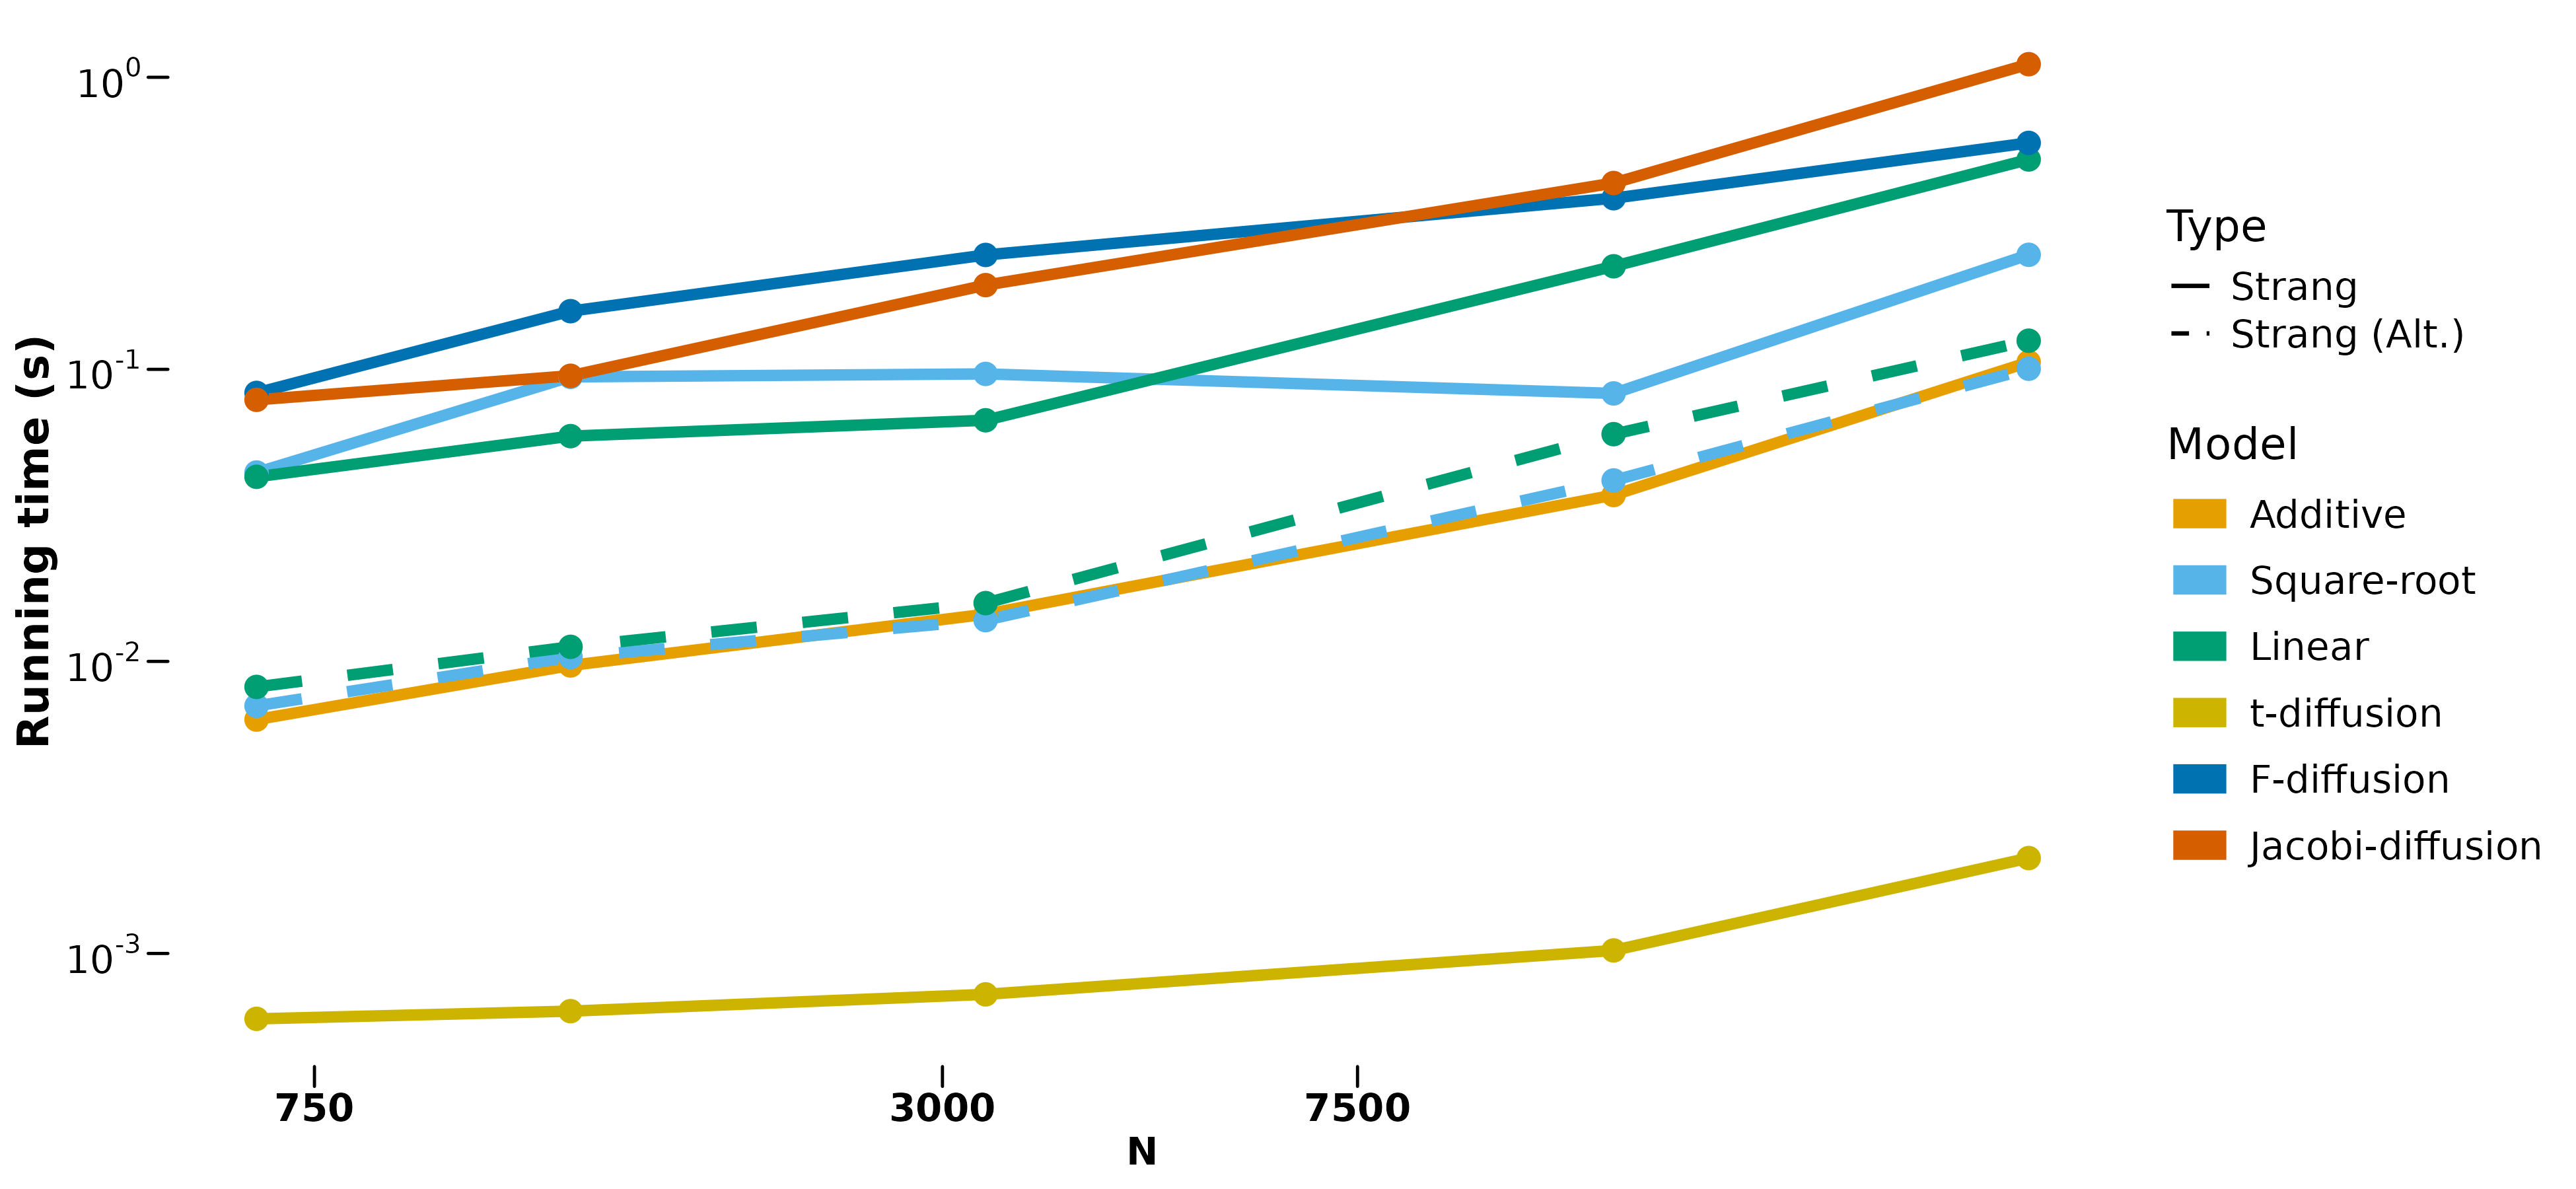
\includegraphics[scale = .1]{figures/estimation_duration_dynamic.jpeg}
    \caption{The median run-time from invokation to convergence in the dynamic part. The ARE of the estimators are shown in figure \ref{figure:parameter_precision_dynamic}}
    \label{figure:estimation_duration_dynamic}
    \end{center}
\end{figure}

\begin{figure}[h!]
    \begin{center}
    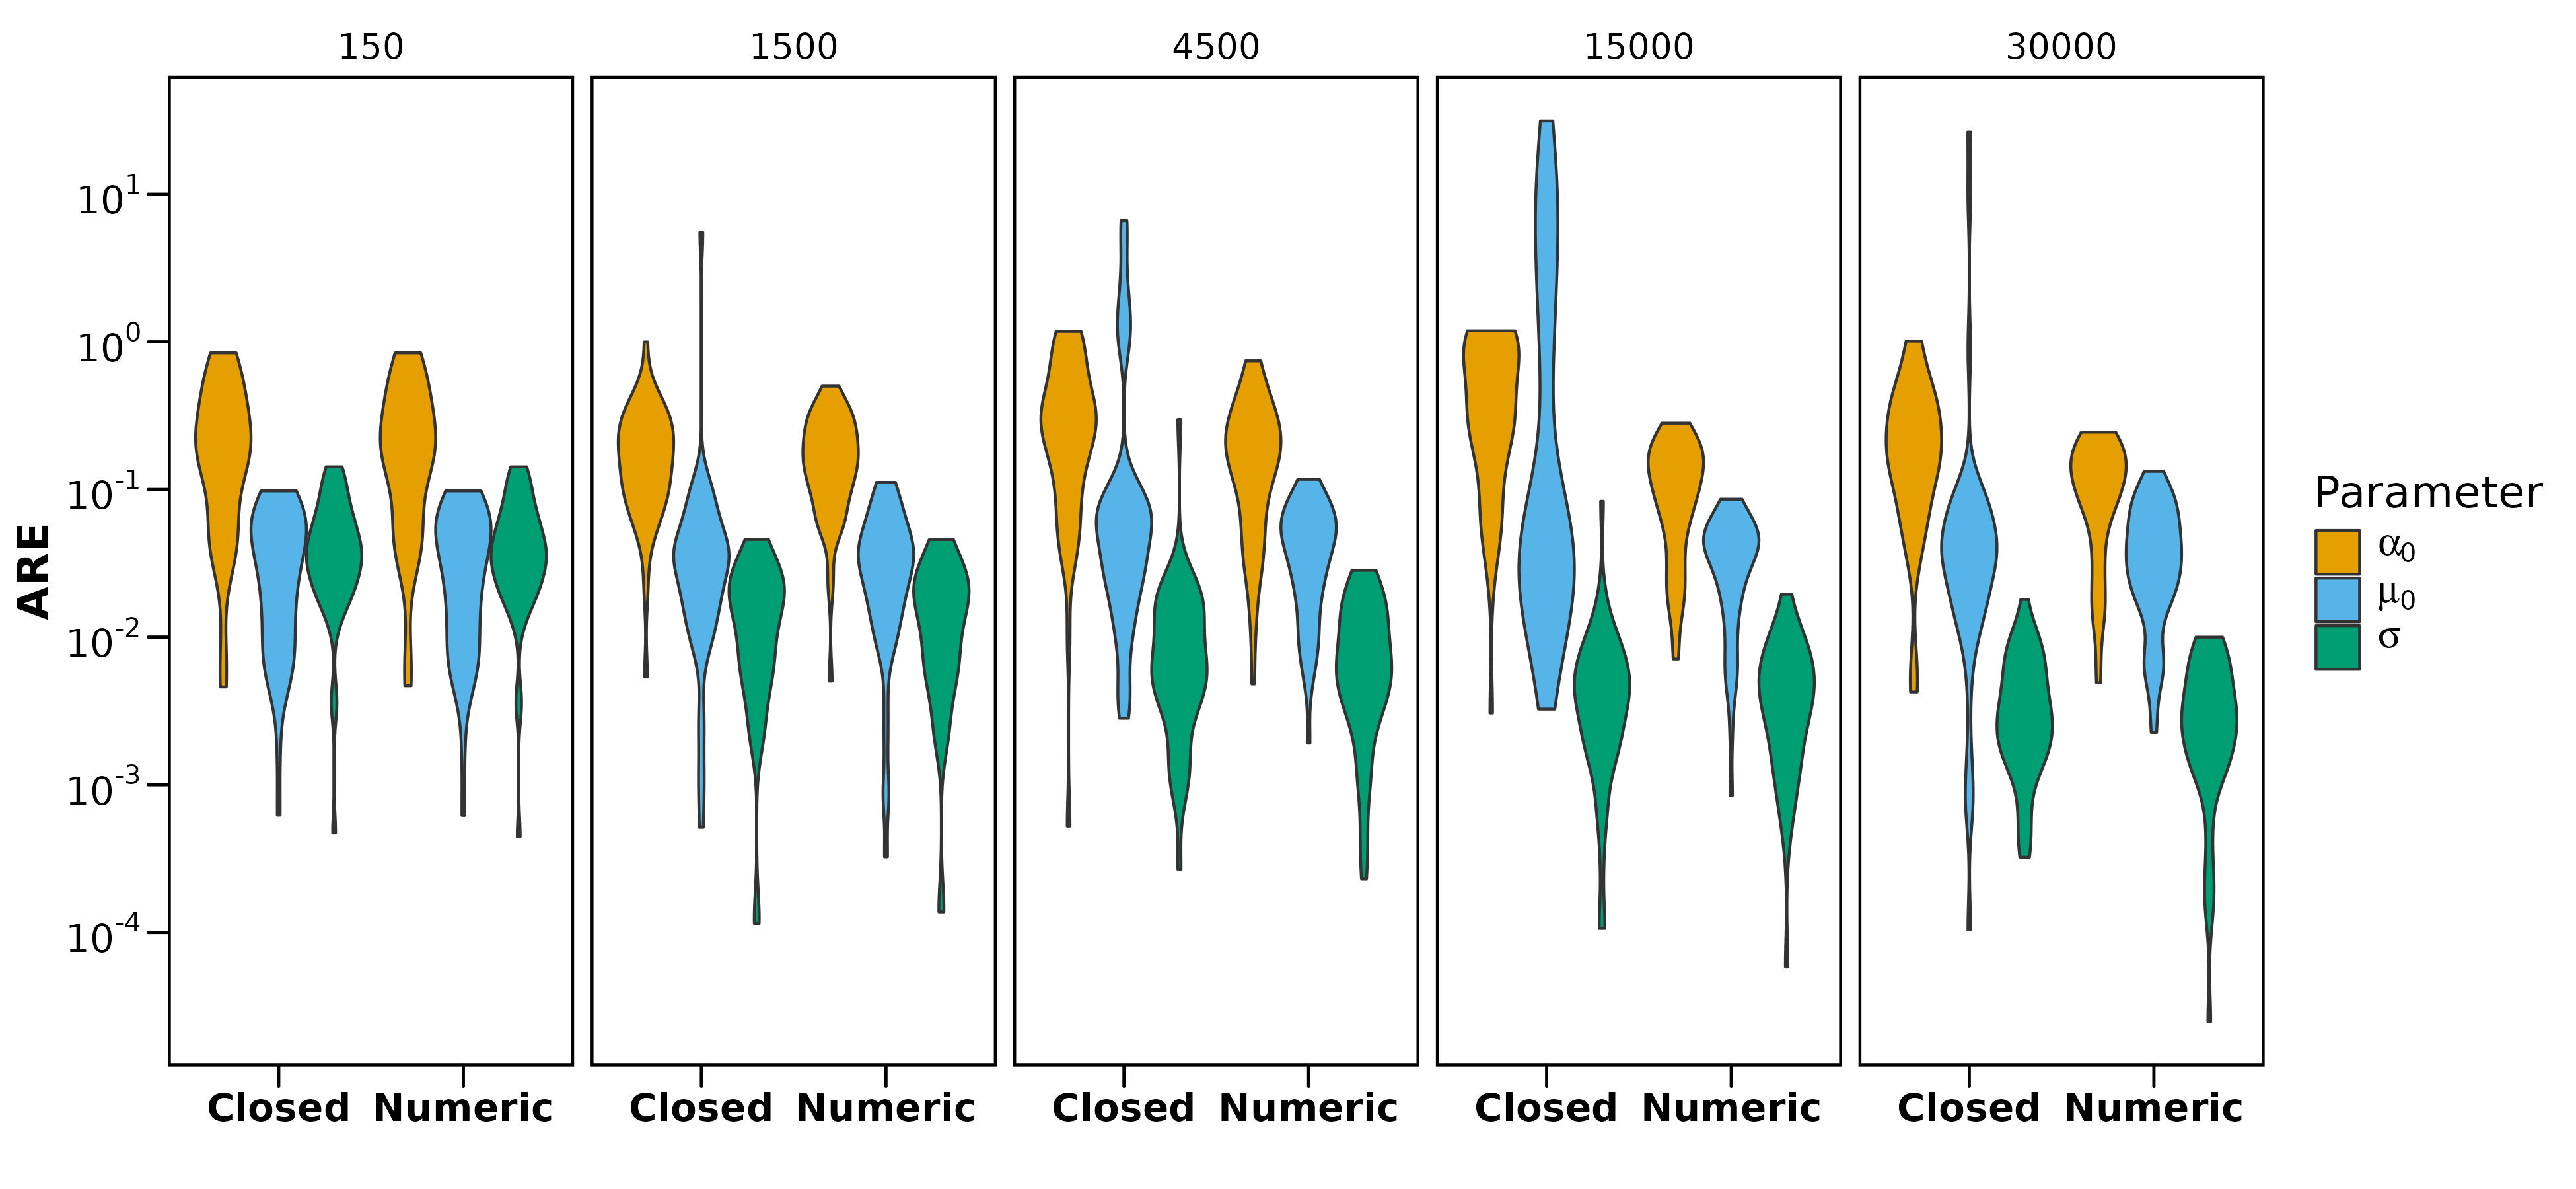
\includegraphics[scale = .1]{figures/ARE_dist_result_plot_F.jpeg}
    \caption{Distribution of the ARE of the parameters in the $F$-diffusion based model shown for the numeric and closed form type estimation methds. A similar result for the linear noise model is shown in figure \ref{figure:ARE_dist_linear_noise}}
    \label{figure:ARE_dist_numeric_F_diffusion}
    \end{center}
\end{figure}

\begin{figure}[h!]
    \begin{center}
    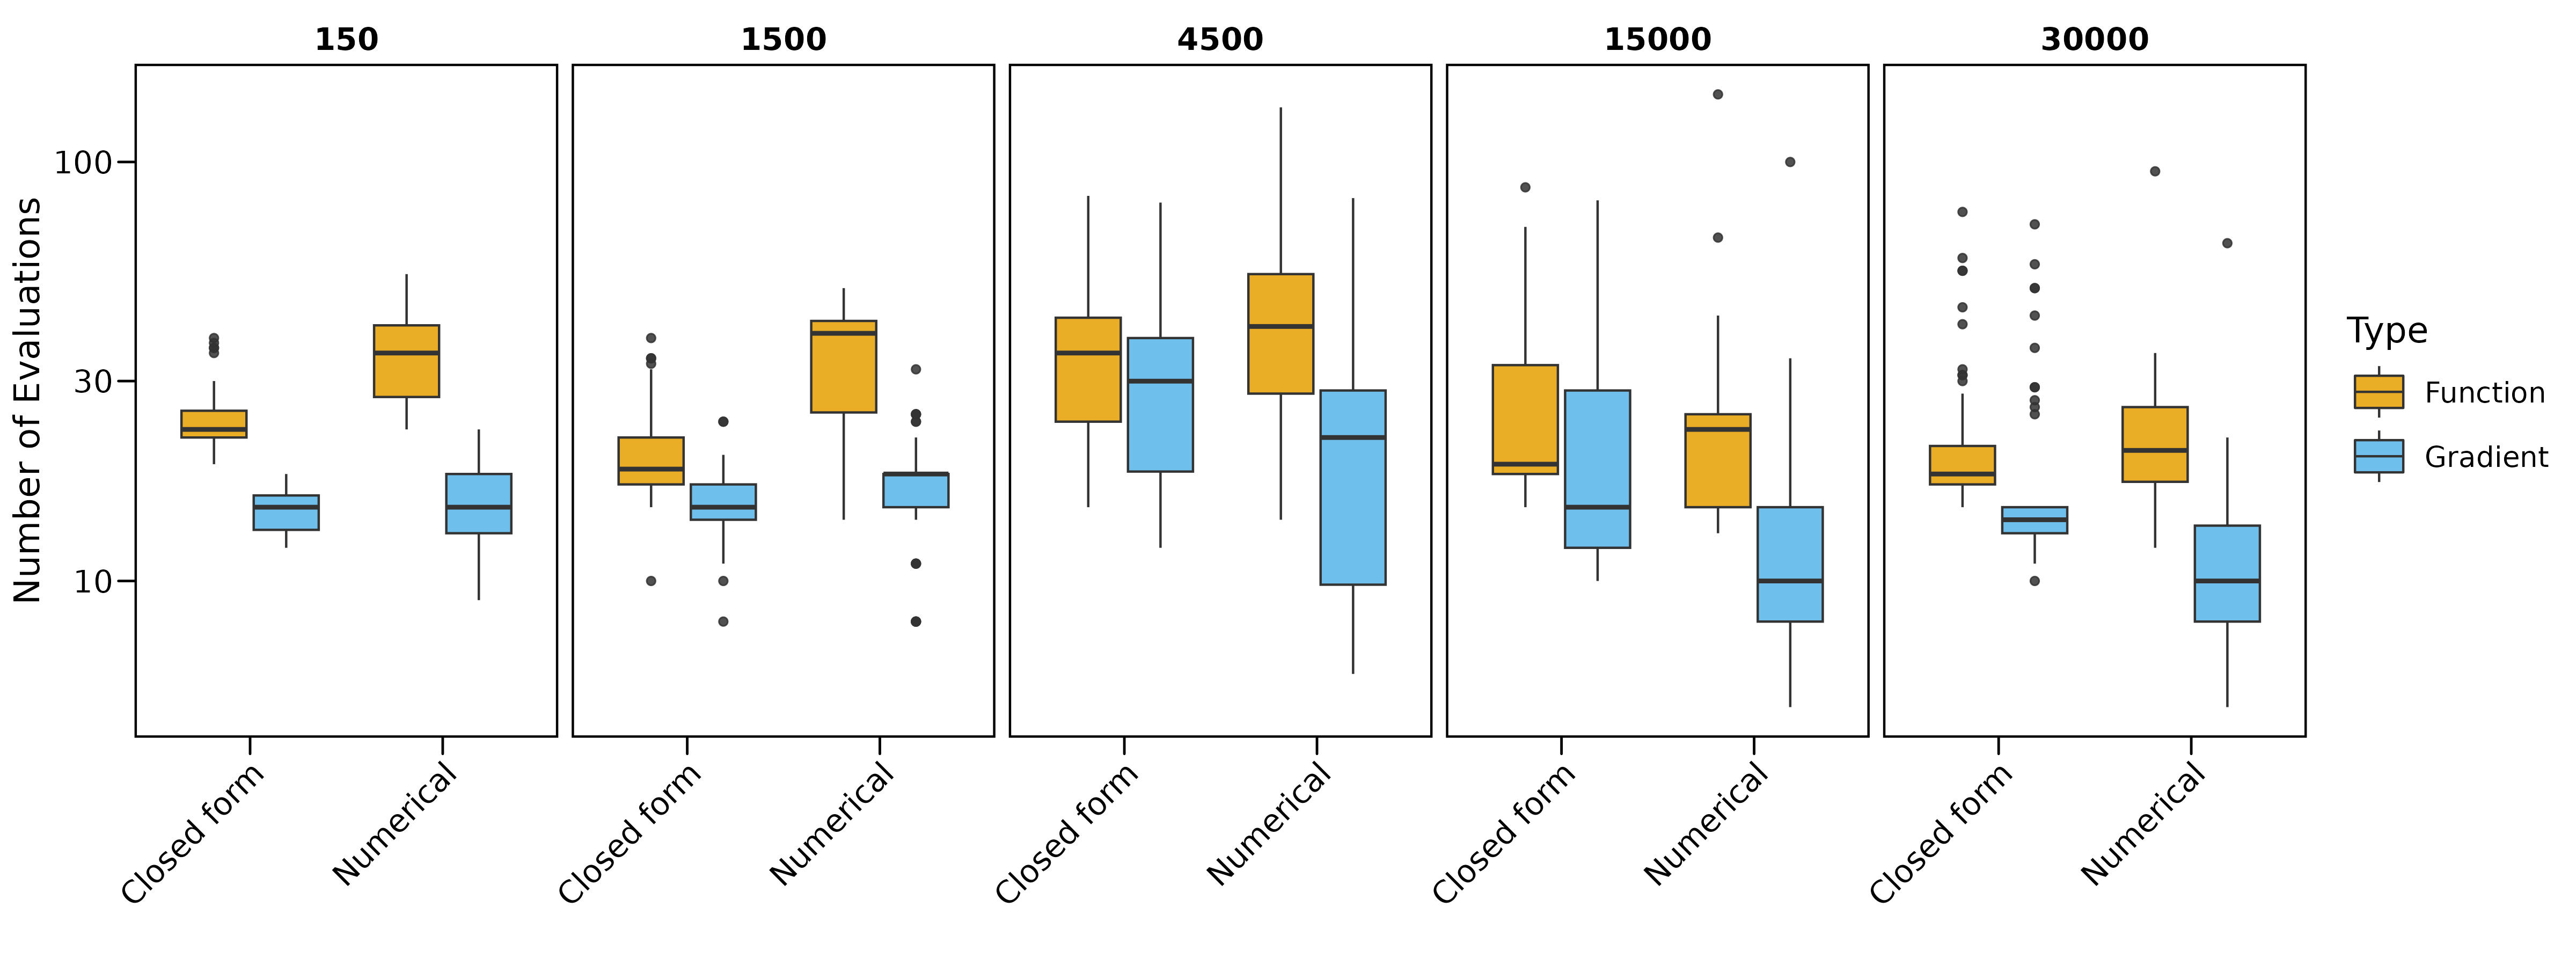
\includegraphics[scale = .08]{figures/function_gradient_count_F_plot.jpeg}     
    \caption{Number of gradient- and function evaluations for the two methods in the experiment on the $F$-diffusion based model. A similar result for the linear-noise model is shown in figure \ref{figure:linearFunctionGradientCount}.}
    \label{figure:FFunctionGradientCount}   
    \end{center}
\end{figure}
\begin{table}[h!]
    \centering
    \begin{tabular}{rrrr}
    $\tau$ & Additive & $t$-diffusion \\ 
      \hline
      $35$ &  $52$ & $112$ \\ 
      $60$ &   $4$ & $6$ \\ 
      $90$ &   $4$ & $1$ \\ 
      $132$ &  $5$ & $3$ \\ 
      $175$ &  $5$ & $0$ \\ 
      $200$ &  $9$ & $0$ \\ 
      $250$ &  $4$ & $0$ \\ 
       \hline
    \end{tabular}
    \caption{Overview of how many times each model had an absolute relative error of above 1.5 stratified after $\tau$ in relation to the simulation study on model misspecification}
    \label{table:AREabove1.5tauSim}
    \end{table}
\newpage
    \subsection{Results}
    In this section we provide supporting information to the results section. Tabels and figures are illustrated in the order they appear in the original section

    \begin{table}[h!]
        \centering
        \begin{tabular}{rllrrrrrrrrr}
          \hline
         Part & $t_0$ & 0.01 & 0.025 & 0.167 & 0.33 & 0.5 & 0.67 & 0.833 & 0.975 & 0.99 \\ 
          \hline
        Theoretical & - & -2.33 & -1.96 & -0.97 & -0.44 & 0.00 & 0.44 & 0.97 & 1.96 & 2.33 \\ 
        Stationary part & 1912 & -2.49 & -2.03 & -0.94 & -0.38 & 0.06 & 0.45 & 0.88 & 1.94 & 2.17 \\ 
        Stationary part & 1924 & -2.43 & -1.99 & -0.90 & -0.41 & 0.02 & 0.44 & 0.89 & 1.96 & 2.42 \\ 
        Dynamic part & 1912 & -2.20 & -1.79 & -0.92 & -0.44 & -0.06 & 0.35 & 0.88 & 2.09 & 2.52 \\ 
        Dynamic part & 1924 & -2.20 & -1.75 & -0.91 & -0.43 & -0.04 & 0.35 & 0.86 & 2.09 & 2.45 \\ 
           \hline
        \end{tabular}
        \caption{Tabularization of the quantiles at selected values for the stationary- and dynamic parts grouped by the $t_0$ used along with the standard normal quantiles. Supports figure \ref{figure:AMOC_QQ_t_0}}
        \label{table:QQ_table_parts}
        \end{table}
    
    \begin{table}[ht]
        \centering
        \begin{tabular}{rrrrrrrrr}
            \hline
            $A$ & $\alpha_0$ & $\lambda_0$ & $m$ & $\mu_0$ & $\sigma$ & $\tau_c$ & Tipping year \\ 
            \hline
            $0.26$ & $3.87$ & $-14.48$ & $-7.24$ & $0.25$ & $0.51$ & $453.29$ & $2377.29$ \\ 
            $0.30$ & $3.63$ & $-11.17$ & $-5.90$ & $0.24$ & $0.53$ & $391.05$ & $2315.05$ \\ 
            $0.27$ & $3.17$ & $-9.33$ & $-5.64$ & $0.24$ & $0.51$ & $383.59$ & $2307.59$ \\ 
            $0.26$ & $3.02$ & $-8.79$ & $-5.63$ & $0.19$ & $0.50$ & $402.94$ & $2326.94$ \\ 
            $0.25$ & $2.92$ & $-8.48$ & $-5.61$ & $0.19$ & $0.52$ & $426.83$ & $2350.83$ \\ 
            $0.32$ & $3.27$ & $-8.42$ & $-4.91$ & $0.24$ & $0.51$ & $348.77$ & $2272.77$ \\ 
            $290.17$ & $2.71$ & $-0.01$ & $0.24$& $0.25$ & $0.48$ & $197.33$ & $2121.33$ \\ 
             \hline
        \end{tabular}
        \caption{Table of estimates that were removed. The reason behind the removing of the estimate has been bolded - though in any case the $m$-estimate is also rather extreme in comparison with the typical distribution in figure \ref{figure:AMOC_parametric_bootstrap}}
        \label{table:extreme_amoc_estimates}
        \end{table}